\PassOptionsToPackage{unicode=true}{hyperref} % options for packages loaded elsewhere
\PassOptionsToPackage{hyphens}{url}
%
\documentclass[12pt,]{article}
\usepackage{lmodern}
\usepackage{amssymb,amsmath}
\usepackage{ifxetex,ifluatex}
\usepackage{fixltx2e} % provides \textsubscript
\ifnum 0\ifxetex 1\fi\ifluatex 1\fi=0 % if pdftex
  \usepackage[T1]{fontenc}
  \usepackage[utf8]{inputenc}
  \usepackage{textcomp} % provides euro and other symbols
\else % if luatex or xelatex
  \usepackage{unicode-math}
  \defaultfontfeatures{Ligatures=TeX,Scale=MatchLowercase}
\fi
% use upquote if available, for straight quotes in verbatim environments
\IfFileExists{upquote.sty}{\usepackage{upquote}}{}
% use microtype if available
\IfFileExists{microtype.sty}{%
\usepackage[]{microtype}
\UseMicrotypeSet[protrusion]{basicmath} % disable protrusion for tt fonts
}{}
\IfFileExists{parskip.sty}{%
\usepackage{parskip}
}{% else
\setlength{\parindent}{0pt}
\setlength{\parskip}{6pt plus 2pt minus 1pt}
}
\usepackage{hyperref}
\hypersetup{
            pdftitle={OBIS extractions from Large Marine Ecosystem regions},
            pdfauthor={Enrique Montes},
            pdfborder={0 0 0},
            breaklinks=true}
\urlstyle{same}  % don't use monospace font for urls
\usepackage[margin=1in]{geometry}
\usepackage{color}
\usepackage{fancyvrb}
\newcommand{\VerbBar}{|}
\newcommand{\VERB}{\Verb[commandchars=\\\{\}]}
\DefineVerbatimEnvironment{Highlighting}{Verbatim}{commandchars=\\\{\}}
% Add ',fontsize=\small' for more characters per line
\usepackage{framed}
\definecolor{shadecolor}{RGB}{248,248,248}
\newenvironment{Shaded}{\begin{snugshade}}{\end{snugshade}}
\newcommand{\AlertTok}[1]{\textcolor[rgb]{0.94,0.16,0.16}{#1}}
\newcommand{\AnnotationTok}[1]{\textcolor[rgb]{0.56,0.35,0.01}{\textbf{\textit{#1}}}}
\newcommand{\AttributeTok}[1]{\textcolor[rgb]{0.77,0.63,0.00}{#1}}
\newcommand{\BaseNTok}[1]{\textcolor[rgb]{0.00,0.00,0.81}{#1}}
\newcommand{\BuiltInTok}[1]{#1}
\newcommand{\CharTok}[1]{\textcolor[rgb]{0.31,0.60,0.02}{#1}}
\newcommand{\CommentTok}[1]{\textcolor[rgb]{0.56,0.35,0.01}{\textit{#1}}}
\newcommand{\CommentVarTok}[1]{\textcolor[rgb]{0.56,0.35,0.01}{\textbf{\textit{#1}}}}
\newcommand{\ConstantTok}[1]{\textcolor[rgb]{0.00,0.00,0.00}{#1}}
\newcommand{\ControlFlowTok}[1]{\textcolor[rgb]{0.13,0.29,0.53}{\textbf{#1}}}
\newcommand{\DataTypeTok}[1]{\textcolor[rgb]{0.13,0.29,0.53}{#1}}
\newcommand{\DecValTok}[1]{\textcolor[rgb]{0.00,0.00,0.81}{#1}}
\newcommand{\DocumentationTok}[1]{\textcolor[rgb]{0.56,0.35,0.01}{\textbf{\textit{#1}}}}
\newcommand{\ErrorTok}[1]{\textcolor[rgb]{0.64,0.00,0.00}{\textbf{#1}}}
\newcommand{\ExtensionTok}[1]{#1}
\newcommand{\FloatTok}[1]{\textcolor[rgb]{0.00,0.00,0.81}{#1}}
\newcommand{\FunctionTok}[1]{\textcolor[rgb]{0.00,0.00,0.00}{#1}}
\newcommand{\ImportTok}[1]{#1}
\newcommand{\InformationTok}[1]{\textcolor[rgb]{0.56,0.35,0.01}{\textbf{\textit{#1}}}}
\newcommand{\KeywordTok}[1]{\textcolor[rgb]{0.13,0.29,0.53}{\textbf{#1}}}
\newcommand{\NormalTok}[1]{#1}
\newcommand{\OperatorTok}[1]{\textcolor[rgb]{0.81,0.36,0.00}{\textbf{#1}}}
\newcommand{\OtherTok}[1]{\textcolor[rgb]{0.56,0.35,0.01}{#1}}
\newcommand{\PreprocessorTok}[1]{\textcolor[rgb]{0.56,0.35,0.01}{\textit{#1}}}
\newcommand{\RegionMarkerTok}[1]{#1}
\newcommand{\SpecialCharTok}[1]{\textcolor[rgb]{0.00,0.00,0.00}{#1}}
\newcommand{\SpecialStringTok}[1]{\textcolor[rgb]{0.31,0.60,0.02}{#1}}
\newcommand{\StringTok}[1]{\textcolor[rgb]{0.31,0.60,0.02}{#1}}
\newcommand{\VariableTok}[1]{\textcolor[rgb]{0.00,0.00,0.00}{#1}}
\newcommand{\VerbatimStringTok}[1]{\textcolor[rgb]{0.31,0.60,0.02}{#1}}
\newcommand{\WarningTok}[1]{\textcolor[rgb]{0.56,0.35,0.01}{\textbf{\textit{#1}}}}
\usepackage{graphicx,grffile}
\makeatletter
\def\maxwidth{\ifdim\Gin@nat@width>\linewidth\linewidth\else\Gin@nat@width\fi}
\def\maxheight{\ifdim\Gin@nat@height>\textheight\textheight\else\Gin@nat@height\fi}
\makeatother
% Scale images if necessary, so that they will not overflow the page
% margins by default, and it is still possible to overwrite the defaults
% using explicit options in \includegraphics[width, height, ...]{}
\setkeys{Gin}{width=\maxwidth,height=\maxheight,keepaspectratio}
\setlength{\emergencystretch}{3em}  % prevent overfull lines
\providecommand{\tightlist}{%
  \setlength{\itemsep}{0pt}\setlength{\parskip}{0pt}}
\setcounter{secnumdepth}{0}
% Redefines (sub)paragraphs to behave more like sections
\ifx\paragraph\undefined\else
\let\oldparagraph\paragraph
\renewcommand{\paragraph}[1]{\oldparagraph{#1}\mbox{}}
\fi
\ifx\subparagraph\undefined\else
\let\oldsubparagraph\subparagraph
\renewcommand{\subparagraph}[1]{\oldsubparagraph{#1}\mbox{}}
\fi

% set default figure placement to htbp
\makeatletter
\def\fps@figure{htbp}
\makeatother

\usepackage{etoolbox}
\makeatletter
\providecommand{\subtitle}[1]{% add subtitle to \maketitle
  \apptocmd{\@title}{\par {\large #1 \par}}{}{}
}
\makeatother
\usepackage{amsmath} \usepackage{color}
% https://github.com/rstudio/rmarkdown/issues/337
\let\rmarkdownfootnote\footnote%
\def\footnote{\protect\rmarkdownfootnote}

% https://github.com/rstudio/rmarkdown/pull/252
\usepackage{titling}
\setlength{\droptitle}{-2em}

\pretitle{\vspace{\droptitle}\centering\huge}
\posttitle{\par}

\preauthor{\centering\large\emph}
\postauthor{\par}

\predate{\centering\large\emph}
\postdate{\par}

\title{OBIS extractions from Large Marine Ecosystem regions}
\author{Enrique Montes}
\date{August 28, 2020}

\begin{document}
\maketitle

\hypertarget{marine-biodiversity-observation-network-pole-to-pole-of-the-americas-mbon-pole-to-pole}{%
\section{\texorpdfstring{Marine Biodiversity Observation Network Pole to
Pole of the Americas (\href{https://marinebon.org/p2p/}{MBON Pole to
Pole})}{Marine Biodiversity Observation Network Pole to Pole of the Americas (MBON Pole to Pole)}}\label{marine-biodiversity-observation-network-pole-to-pole-of-the-americas-mbon-pole-to-pole}}

This code creates a map showing the boundaries of a selected Large
Marine Ecosystems
(\href{http://lme.edc.uri.edu/index.php/lme-introduction}{LME}) and
extracts records for selected taxa from the
\href{https://obis.org/}{Ocean Biodiversity Information System (OBIS)}
using \href{https://obis.org/manual/accessr/}{robis} tools.

\hypertarget{first-lets-load-required-libraries}{%
\section{First, let's load required
libraries}\label{first-lets-load-required-libraries}}

\begin{Shaded}
\begin{Highlighting}[]
\KeywordTok{library}\NormalTok{(robis)}
\end{Highlighting}
\end{Shaded}

\begin{verbatim}
## Warning: package 'robis' was built under R version 3.6.2
\end{verbatim}

\begin{Shaded}
\begin{Highlighting}[]
\KeywordTok{library}\NormalTok{(rgdal) }\CommentTok{# for `ogrInfo()` and `readOGR()`}
\end{Highlighting}
\end{Shaded}

\begin{verbatim}
## Warning: package 'rgdal' was built under R version 3.6.2
\end{verbatim}

\begin{verbatim}
## Loading required package: sp
\end{verbatim}

\begin{verbatim}
## rgdal: version: 1.5-16, (SVN revision 1050)
## Geospatial Data Abstraction Library extensions to R successfully loaded
## Loaded GDAL runtime: GDAL 2.4.2, released 2019/06/28
## Path to GDAL shared files: /Users/enriquemontes/Library/R/3.6/library/rgdal/gdal
## GDAL binary built with GEOS: FALSE 
## Loaded PROJ runtime: Rel. 5.2.0, September 15th, 2018, [PJ_VERSION: 520]
## Path to PROJ shared files: /Users/enriquemontes/Library/R/3.6/library/rgdal/proj
## Linking to sp version:1.4-2
## Overwritten PROJ_LIB was /Users/enriquemontes/Library/R/3.6/library/rgdal/proj
\end{verbatim}

\begin{Shaded}
\begin{Highlighting}[]
\KeywordTok{library}\NormalTok{(tools) }\CommentTok{# for `file_path_sans_ext()`}
\KeywordTok{library}\NormalTok{(dplyr) }\CommentTok{# for `inner_join()`, `filter()`, `summarise()`, and the pipe operator (%>%)}
\end{Highlighting}
\end{Shaded}

\begin{verbatim}
## 
## Attaching package: 'dplyr'
\end{verbatim}

\begin{verbatim}
## The following objects are masked from 'package:stats':
## 
##     filter, lag
\end{verbatim}

\begin{verbatim}
## The following objects are masked from 'package:base':
## 
##     intersect, setdiff, setequal, union
\end{verbatim}

\begin{Shaded}
\begin{Highlighting}[]
\KeywordTok{library}\NormalTok{(ggplot2) }\CommentTok{# for `fortify()` and for plotting}
\KeywordTok{library}\NormalTok{(sp) }\CommentTok{# for `point.in.polygon()` and `spDists()`}
\KeywordTok{library}\NormalTok{(tidyr) }\CommentTok{# for `gather()`}
\KeywordTok{library}\NormalTok{(readr) }\CommentTok{# for `write_tsv()`}
\KeywordTok{library}\NormalTok{(leaflet)}
\KeywordTok{library}\NormalTok{(lubridate)}
\end{Highlighting}
\end{Shaded}

\begin{verbatim}
## 
## Attaching package: 'lubridate'
\end{verbatim}

\begin{verbatim}
## The following object is masked from 'package:base':
## 
##     date
\end{verbatim}

\hypertarget{now-lets-provide-the-function-fortify.shape-which-puts-the-shapefile-data-in-the-object-class-data.frame-so-that-it-can-be-used-by-ggplot2-and-extract-portions-of-the-data-from-the-fortified-data.frame-object-for-a-smaller-domain}{%
\subsection{Now let's provide the function fortify.shape(), which puts
the shapefile data in the object class data.frame, so that it can be
used by ggplot2, and extract portions of the data (from the fortified
data.frame object) for a smaller
domain}\label{now-lets-provide-the-function-fortify.shape-which-puts-the-shapefile-data-in-the-object-class-data.frame-so-that-it-can-be-used-by-ggplot2-and-extract-portions-of-the-data-from-the-fortified-data.frame-object-for-a-smaller-domain}}

\begin{Shaded}
\begin{Highlighting}[]
\NormalTok{fortify.shape <-}\StringTok{ }\ControlFlowTok{function}\NormalTok{(x)\{}
\NormalTok{  x}\OperatorTok{@}\NormalTok{data}\OperatorTok{$}\NormalTok{id <-}\StringTok{ }\KeywordTok{rownames}\NormalTok{(x}\OperatorTok{@}\NormalTok{data)}
\NormalTok{  x.f <-}\StringTok{ }\KeywordTok{fortify}\NormalTok{(x, }\DataTypeTok{region =} \StringTok{"id"}\NormalTok{)}
\NormalTok{  x.join <-}\StringTok{ }\KeywordTok{inner_join}\NormalTok{(x.f, x}\OperatorTok{@}\NormalTok{data, }\DataTypeTok{by =} \StringTok{"id"}\NormalTok{)}
\NormalTok{\}}

\NormalTok{subset.shape <-}\StringTok{ }\ControlFlowTok{function}\NormalTok{(x, domain)\{}
\NormalTok{  x.subset <-}\StringTok{ }\KeywordTok{filter}\NormalTok{(x, long }\OperatorTok{>}\StringTok{ }\NormalTok{domain[}\DecValTok{1}\NormalTok{] }\OperatorTok{&}\StringTok{ }
\StringTok{                       }\NormalTok{long }\OperatorTok{<}\StringTok{ }\NormalTok{domain[}\DecValTok{2}\NormalTok{] }\OperatorTok{&}\StringTok{ }
\StringTok{                       }\NormalTok{lat }\OperatorTok{>}\StringTok{ }\NormalTok{domain[}\DecValTok{3}\NormalTok{] }\OperatorTok{&}\StringTok{ }
\StringTok{                       }\NormalTok{lat }\OperatorTok{<}\StringTok{ }\NormalTok{domain[}\DecValTok{4}\NormalTok{])}
\NormalTok{  x.subset}
\NormalTok{\}}
\end{Highlighting}
\end{Shaded}

Let's read the shapefile ``LMEs66.shp'' containing all polygons, fortify
the global data and then extract domain. See numbers
\href{http://lme.edc.uri.edu/index.php/lme-introduction}{here}

\begin{Shaded}
\begin{Highlighting}[]
\NormalTok{path.lme.coast <-}\StringTok{ }\NormalTok{(}\StringTok{"~/lme-extractions/data"}\NormalTok{)}
\NormalTok{fnam.lme.coast <-}\StringTok{ "LMEs66.shp"}
\NormalTok{dat.coast <-}\StringTok{ }\KeywordTok{readOGR}\NormalTok{(}\DataTypeTok{dsn =}\NormalTok{ path.lme.coast, }
                     \DataTypeTok{layer =} \KeywordTok{file_path_sans_ext}\NormalTok{(fnam.lme.coast))}
\end{Highlighting}
\end{Shaded}

\begin{verbatim}
## OGR data source with driver: ESRI Shapefile 
## Source: "/Users/enriquemontes/lme-extractions/data", layer: "LMEs66"
## with 66 features
## It has 9 fields
## Integer64 fields read as strings:  OBJECTID
\end{verbatim}

\begin{Shaded}
\begin{Highlighting}[]
\CommentTok{# fortify the global data and then extract domain}
\NormalTok{dat.coast <-}\StringTok{ }\KeywordTok{fortify.shape}\NormalTok{(dat.coast) }\CommentTok{# a 410951x8 dataframe}
\end{Highlighting}
\end{Shaded}

\begin{verbatim}
## Warning in RGEOSUnaryPredFunc(spgeom, byid, "rgeos_isvalid"): Ring Self-
## intersection at or near point 10.97943974 54.380550380000003
\end{verbatim}

\begin{verbatim}
## Warning in RGEOSUnaryPredFunc(spgeom, byid, "rgeos_isvalid"): Self-intersection
## at or near point 103.91529846 10.28388977
\end{verbatim}

\begin{verbatim}
## Warning in RGEOSUnaryPredFunc(spgeom, byid, "rgeos_isvalid"): Ring Self-
## intersection at or near point -161.34730529999999 58.665809629999998
\end{verbatim}

\begin{verbatim}
## SpP is invalid
\end{verbatim}

\begin{verbatim}
## Warning in rgeos::gUnaryUnion(spgeom = SpP, id = IDs): Invalid objects found;
## consider using set_RGEOS_CheckValidity(2L)
\end{verbatim}

\begin{Shaded}
\begin{Highlighting}[]
\CommentTok{# Specify the desired LME:}
\NormalTok{dat.sel_}\DecValTok{1}\NormalTok{ <-}\StringTok{ }\KeywordTok{subset}\NormalTok{(dat.coast, LME_NUMBER }\OperatorTok{==}\StringTok{ }\DecValTok{15}\NormalTok{) }\CommentTok{# S. Brazil. }
\NormalTok{dat.sel_}\DecValTok{2}\NormalTok{ <-}\StringTok{ }\KeywordTok{subset}\NormalTok{(dat.coast, LME_NUMBER }\OperatorTok{==}\StringTok{ }\DecValTok{16}\NormalTok{) }\CommentTok{# E. Brazil}
\NormalTok{dat.sel_}\DecValTok{3}\NormalTok{ <-}\StringTok{ }\KeywordTok{subset}\NormalTok{(dat.coast, LME_NUMBER }\OperatorTok{==}\StringTok{ }\DecValTok{17}\NormalTok{) }\CommentTok{# N. Brazil}
\NormalTok{dat.sel_}\DecValTok{4}\NormalTok{ <-}\StringTok{ }\KeywordTok{subset}\NormalTok{(dat.coast, LME_NUMBER }\OperatorTok{==}\StringTok{ }\DecValTok{14}\NormalTok{) }\CommentTok{# Patagonia}
\NormalTok{dat.sel_}\DecValTok{5}\NormalTok{ <-}\StringTok{ }\KeywordTok{subset}\NormalTok{(dat.coast, LME_NUMBER }\OperatorTok{==}\StringTok{ }\DecValTok{13}\NormalTok{) }\CommentTok{# Humboldt C.}
\NormalTok{dat.sel_}\DecValTok{6}\NormalTok{ <-}\StringTok{ }\KeywordTok{subset}\NormalTok{(dat.coast, LME_NUMBER }\OperatorTok{==}\StringTok{ }\DecValTok{12}\NormalTok{) }\CommentTok{# Caribbean}
\NormalTok{dat.sel_}\DecValTok{7}\NormalTok{ <-}\StringTok{ }\KeywordTok{subset}\NormalTok{(dat.coast, LME_NUMBER }\OperatorTok{==}\StringTok{ }\DecValTok{11}\NormalTok{) }\CommentTok{# P. Ctral A.}
\NormalTok{dat.sel_}\DecValTok{8}\NormalTok{ <-}\StringTok{ }\KeywordTok{subset}\NormalTok{(dat.coast, LME_NUMBER }\OperatorTok{==}\StringTok{ }\DecValTok{5}\NormalTok{) }\CommentTok{# GoM}
\NormalTok{dat.sel_}\DecValTok{9}\NormalTok{ <-}\StringTok{ }\KeywordTok{subset}\NormalTok{(dat.coast, LME_NUMBER }\OperatorTok{==}\StringTok{ }\DecValTok{4}\NormalTok{) }\CommentTok{# Gulf of California}
\NormalTok{dat.sel_}\DecValTok{10}\NormalTok{ <-}\StringTok{ }\KeywordTok{subset}\NormalTok{(dat.coast, LME_NUMBER }\OperatorTok{==}\StringTok{ }\DecValTok{3}\NormalTok{) }\CommentTok{# CCS}
\NormalTok{dat.sel_}\DecValTok{11}\NormalTok{ <-}\StringTok{ }\KeywordTok{subset}\NormalTok{(dat.coast, LME_NUMBER }\OperatorTok{==}\StringTok{ }\DecValTok{2}\NormalTok{) }\CommentTok{# G. Alaska}
\NormalTok{dat.sel_}\DecValTok{12}\NormalTok{ <-}\StringTok{ }\KeywordTok{subset}\NormalTok{(dat.coast, LME_NUMBER }\OperatorTok{==}\StringTok{ }\DecValTok{1}\NormalTok{) }\CommentTok{# E. Bearing S.}
\NormalTok{dat.sel_}\DecValTok{13}\NormalTok{ <-}\StringTok{ }\KeywordTok{subset}\NormalTok{(dat.coast, LME_NUMBER }\OperatorTok{==}\StringTok{ }\DecValTok{54}\NormalTok{) }\CommentTok{# Chukchi S.}
\NormalTok{dat.sel_}\DecValTok{14}\NormalTok{ <-}\StringTok{ }\KeywordTok{subset}\NormalTok{(dat.coast, LME_NUMBER }\OperatorTok{==}\StringTok{ }\DecValTok{55}\NormalTok{) }\CommentTok{# Beauford S.}
\NormalTok{dat.sel_}\DecValTok{15}\NormalTok{ <-}\StringTok{ }\KeywordTok{subset}\NormalTok{(dat.coast, LME_NUMBER }\OperatorTok{==}\StringTok{ }\DecValTok{66}\NormalTok{) }\CommentTok{# Canadian Arctic}
\NormalTok{dat.sel_}\DecValTok{16}\NormalTok{ <-}\StringTok{ }\KeywordTok{subset}\NormalTok{(dat.coast, LME_NUMBER }\OperatorTok{==}\StringTok{ }\DecValTok{18}\NormalTok{) }\CommentTok{# Canadian E. Arctic}
\NormalTok{dat.sel_}\DecValTok{17}\NormalTok{ <-}\StringTok{ }\KeywordTok{subset}\NormalTok{(dat.coast, LME_NUMBER }\OperatorTok{==}\StringTok{ }\DecValTok{9}\NormalTok{) }\CommentTok{# Labrador S.}
\NormalTok{dat.sel_}\DecValTok{18}\NormalTok{ <-}\StringTok{ }\KeywordTok{subset}\NormalTok{(dat.coast, LME_NUMBER }\OperatorTok{==}\StringTok{ }\DecValTok{8}\NormalTok{) }\CommentTok{# Scotian Shelf}
\NormalTok{dat.sel_}\DecValTok{19}\NormalTok{ <-}\StringTok{ }\KeywordTok{subset}\NormalTok{(dat.coast, LME_NUMBER }\OperatorTok{==}\StringTok{ }\DecValTok{7}\NormalTok{) }\CommentTok{# NE US}
\NormalTok{dat.sel_}\DecValTok{20}\NormalTok{ <-}\StringTok{ }\KeywordTok{subset}\NormalTok{(dat.coast, LME_NUMBER }\OperatorTok{==}\StringTok{ }\DecValTok{6}\NormalTok{) }\CommentTok{# SE US}
\NormalTok{dat.sel_}\DecValTok{21}\NormalTok{ <-}\StringTok{ }\KeywordTok{subset}\NormalTok{(dat.coast, LME_NUMBER }\OperatorTok{==}\StringTok{ }\DecValTok{10}\NormalTok{) }\CommentTok{# Hawaii}
\NormalTok{dat.sel_}\DecValTok{22}\NormalTok{ <-}\StringTok{ }\KeywordTok{subset}\NormalTok{(dat.coast, LME_NUMBER }\OperatorTok{==}\StringTok{ }\DecValTok{63}\NormalTok{) }\CommentTok{# Hudson Bay Complex}
\NormalTok{dat.sel_}\DecValTok{23}\NormalTok{ <-}\StringTok{ }\KeywordTok{subset}\NormalTok{(dat.coast, LME_NUMBER }\OperatorTok{==}\StringTok{ }\DecValTok{19}\NormalTok{) }\CommentTok{# Greenland Sea}
\NormalTok{dat.sel_}\DecValTok{24}\NormalTok{ <-}\StringTok{ }\KeywordTok{subset}\NormalTok{(dat.coast, LME_NUMBER }\OperatorTok{==}\StringTok{ }\DecValTok{21}\NormalTok{) }\CommentTok{# Norwegian Sea}
\NormalTok{dat.sel_}\DecValTok{25}\NormalTok{ <-}\StringTok{ }\KeywordTok{subset}\NormalTok{(dat.coast, LME_NUMBER }\OperatorTok{==}\StringTok{ }\DecValTok{20}\NormalTok{) }\CommentTok{# Barents Sea}
\NormalTok{dat.sel_}\DecValTok{26}\NormalTok{ <-}\StringTok{ }\KeywordTok{subset}\NormalTok{(dat.coast, LME_NUMBER }\OperatorTok{==}\StringTok{ }\DecValTok{58}\NormalTok{) }\CommentTok{# Kara Sea}
\NormalTok{dat.sel_}\DecValTok{27}\NormalTok{ <-}\StringTok{ }\KeywordTok{subset}\NormalTok{(dat.coast, LME_NUMBER }\OperatorTok{==}\StringTok{ }\DecValTok{57}\NormalTok{) }\CommentTok{# Laptev Sea}
\NormalTok{dat.sel_}\DecValTok{28}\NormalTok{ <-}\StringTok{ }\KeywordTok{subset}\NormalTok{(dat.coast, LME_NUMBER }\OperatorTok{==}\StringTok{ }\DecValTok{56}\NormalTok{) }\CommentTok{# E. Sibarian Sea}
\end{Highlighting}
\end{Shaded}

Plotting the coastline and selected LME boundaries

\begin{Shaded}
\begin{Highlighting}[]
\CommentTok{# Define lat/lon limits here}
\NormalTok{xlims <-}\StringTok{ }\KeywordTok{c}\NormalTok{(}\OperatorTok{-}\DecValTok{150}\NormalTok{, }\DecValTok{-25}\NormalTok{)}
\NormalTok{ylims <-}\StringTok{ }\KeywordTok{c}\NormalTok{(}\OperatorTok{-}\DecValTok{60}\NormalTok{, }\DecValTok{60}\NormalTok{)}

\CommentTok{# Generate a base map with the coastline:}
\NormalTok{p0 <-}\StringTok{ }\KeywordTok{ggplot}\NormalTok{() }\OperatorTok{+}\StringTok{ }\KeywordTok{theme}\NormalTok{(}\DataTypeTok{text =} \KeywordTok{element_text}\NormalTok{(}\DataTypeTok{size=}\DecValTok{18}\NormalTok{)) }\OperatorTok{+}\StringTok{ }
\StringTok{  }\KeywordTok{geom_path}\NormalTok{(}\DataTypeTok{data =}\NormalTok{ dat.coast, }\KeywordTok{aes}\NormalTok{(}\DataTypeTok{x =}\NormalTok{ long, }\DataTypeTok{y =}\NormalTok{ lat, }\DataTypeTok{group =}\NormalTok{ group), }
            \DataTypeTok{color =} \StringTok{"black"}\NormalTok{, }\DataTypeTok{size =} \FloatTok{0.25}\NormalTok{) }\OperatorTok{+}\StringTok{ }
\StringTok{  }\KeywordTok{coord_map}\NormalTok{(}\DataTypeTok{projection =} \StringTok{"mercator"}\NormalTok{) }\OperatorTok{+}\StringTok{ }
\StringTok{  }\KeywordTok{scale_x_continuous}\NormalTok{(}\DataTypeTok{limits =}\NormalTok{ xlims, }\DataTypeTok{expand =} \KeywordTok{c}\NormalTok{(}\DecValTok{0}\NormalTok{, }\DecValTok{0}\NormalTok{)) }\OperatorTok{+}\StringTok{ }
\StringTok{  }\KeywordTok{scale_y_continuous}\NormalTok{(}\DataTypeTok{limits =}\NormalTok{ ylims, }\DataTypeTok{expand =} \KeywordTok{c}\NormalTok{(}\DecValTok{0}\NormalTok{, }\DecValTok{0}\NormalTok{)) }\OperatorTok{+}\StringTok{ }
\StringTok{  }\KeywordTok{labs}\NormalTok{(}\KeywordTok{list}\NormalTok{(}\DataTypeTok{title =} \StringTok{""}\NormalTok{, }\DataTypeTok{x =} \StringTok{"Longitude"}\NormalTok{, }\DataTypeTok{y =} \StringTok{"Latitude"}\NormalTok{))}

\NormalTok{p0}
\end{Highlighting}
\end{Shaded}

\begin{verbatim}
## Warning: Removed 495407 rows containing missing values (geom_path).
\end{verbatim}

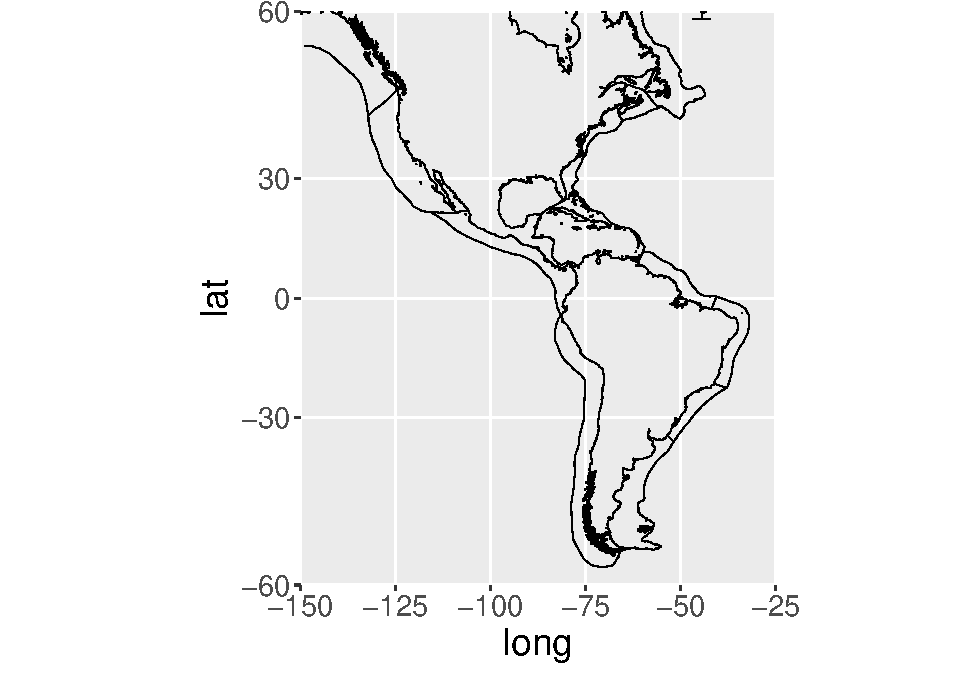
\includegraphics{lme_extractions_files/figure-latex/unnamed-chunk-4-1.pdf}

\begin{Shaded}
\begin{Highlighting}[]
\CommentTok{# highlight LME of interest}
\NormalTok{p.sel <-}\StringTok{ }\NormalTok{p0 }\OperatorTok{+}
\StringTok{  }\KeywordTok{geom_path}\NormalTok{(}\DataTypeTok{data =}\NormalTok{ dat.sel_}\DecValTok{6}\NormalTok{,}
            \KeywordTok{aes}\NormalTok{(}\DataTypeTok{x =}\NormalTok{ long, }\DataTypeTok{y =}\NormalTok{ lat, }\DataTypeTok{group =}\NormalTok{ group),}
            \DataTypeTok{colour =} \StringTok{"chartreuse4"}\NormalTok{, }\DataTypeTok{size =} \DecValTok{1}\NormalTok{) }\OperatorTok{+}
\StringTok{  }\KeywordTok{geom_path}\NormalTok{(}\DataTypeTok{data =}\NormalTok{ dat.sel_}\DecValTok{8}\NormalTok{,}
            \KeywordTok{aes}\NormalTok{(}\DataTypeTok{x =}\NormalTok{ long, }\DataTypeTok{y =}\NormalTok{ lat, }\DataTypeTok{group =}\NormalTok{ group),}
            \DataTypeTok{colour =} \StringTok{"coral"}\NormalTok{, }\DataTypeTok{size =} \FloatTok{0.75}\NormalTok{)}
\NormalTok{p.sel}
\end{Highlighting}
\end{Shaded}

\begin{verbatim}
## Warning: Removed 495407 rows containing missing values (geom_path).
\end{verbatim}

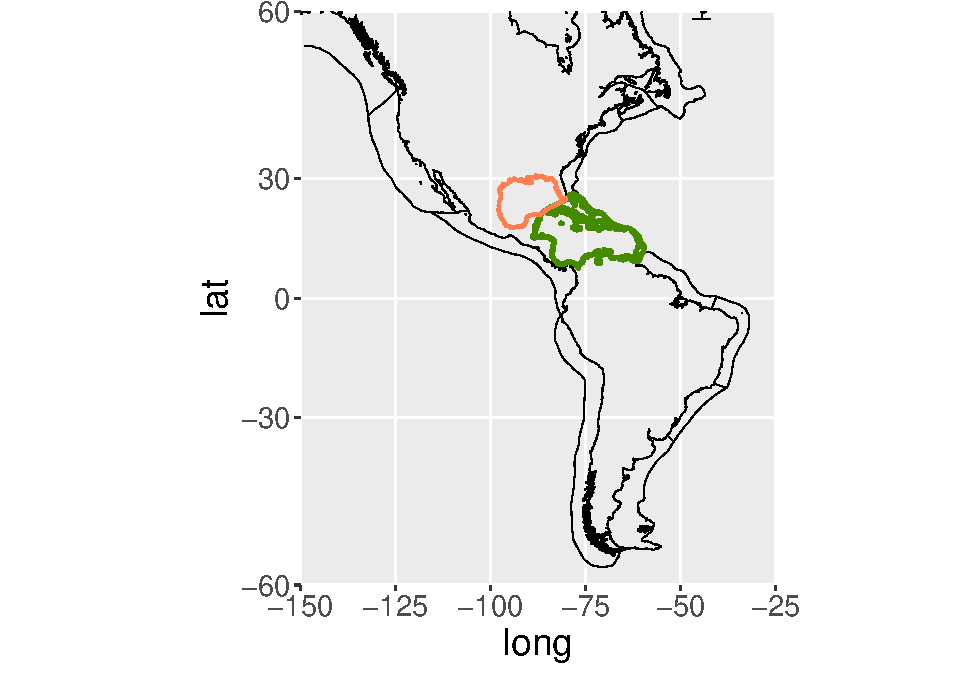
\includegraphics{lme_extractions_files/figure-latex/unnamed-chunk-4-2.pdf}

This section extracts OBIS records of using the ``occurrence'' function
or downloaded data, and plots time series or pie charts with
distributions of large groups (annelids, molluscs, plants and
echinoderms) in the upper 100m.

\begin{Shaded}
\begin{Highlighting}[]
\CommentTok{# Set extraction params}
\CommentTok{# LME codes (from OBIS URL)}
\CommentTok{# N Brazil=40017; E Brazil=40016; S Brazil=40015; Patagonia=40014; Humboldt=40013; Caribbean=40012; }
\CommentTok{# P Ctral A=40011; CCS=40003; GoA=40002; NE USA=40007; E Bearing=40001; Canada E Arctic=40018; GoM=40005; }
\CommentTok{# Chukchi=40054; SE USA=40006; Labrador=40009; Scotian S=40008}

\NormalTok{area =}\StringTok{ }\DecValTok{40005}  
\NormalTok{depth =}\StringTok{ }\DecValTok{100}
\NormalTok{mol_code =}\StringTok{ }\DecValTok{51}
\NormalTok{echi_code =}\StringTok{ }\DecValTok{1806}
\NormalTok{anne_code =}\StringTok{ }\DecValTok{882}
\NormalTok{plan_code =}\StringTok{ }\DecValTok{3}

\CommentTok{## read data from OBIS}
\CommentTok{## Molluscs}
\NormalTok{mollusc}\FloatTok{.100}\NormalTok{_}\DecValTok{2}\NormalTok{ =}\StringTok{ }\KeywordTok{occurrence}\NormalTok{(}\DataTypeTok{areaid =}\NormalTok{ area, }\DataTypeTok{taxonid =}\NormalTok{ mol_code, }\DataTypeTok{enddepth =}\NormalTok{ depth) }
\end{Highlighting}
\end{Shaded}

\begin{verbatim}
## Retrieved 5000 records of approximately 87413 (5%) Retrieved 10000 records of
## approximately 87413 (11%) Retrieved 15000 records of approximately 87413 (17%)
## Retrieved 20000 records of approximately 87413 (22%) Retrieved 25000 records of
## approximately 87413 (28%) Retrieved 30000 records of approximately 87413 (34%)
## Retrieved 35000 records of approximately 87413 (40%) Retrieved 40000 records of
## approximately 87413 (45%) Retrieved 45000 records of approximately 87413 (51%)
## Retrieved 50000 records of approximately 87413 (57%) Retrieved 55000 records of
## approximately 87413 (62%) Retrieved 60000 records of approximately 87413 (68%)
## Retrieved 65000 records of approximately 87413 (74%) Retrieved 70000 records of
## approximately 87413 (80%) Retrieved 75000 records of approximately 87413 (85%)
## Retrieved 80000 records of approximately 87413 (91%) Retrieved 85000 records of
## approximately 87413 (97%) Retrieved 87413 records of approximately 87413 (100%)
\end{verbatim}

\begin{Shaded}
\begin{Highlighting}[]
\CommentTok{## Ehinoderms}
\NormalTok{echino}\FloatTok{.100}\NormalTok{_}\DecValTok{2}\NormalTok{ =}\StringTok{ }\KeywordTok{occurrence}\NormalTok{(}\DataTypeTok{areaid =}\NormalTok{ area, }\DataTypeTok{taxonid =}\NormalTok{ echi_code, }\DataTypeTok{enddepth =}\NormalTok{ depth)}
\end{Highlighting}
\end{Shaded}

\begin{verbatim}
## Retrieved 5000 records of approximately 16811 (29%) Retrieved 10000 records of
## approximately 16811 (59%) Retrieved 15000 records of approximately 16811 (89%)
## Retrieved 16811 records of approximately 16811 (100%)
\end{verbatim}

\begin{Shaded}
\begin{Highlighting}[]
\CommentTok{## Annelida}
\NormalTok{anne}\FloatTok{.100}\NormalTok{_}\DecValTok{2}\NormalTok{ =}\StringTok{ }\KeywordTok{occurrence}\NormalTok{(}\DataTypeTok{areaid =}\NormalTok{ area, }\DataTypeTok{taxonid =}\NormalTok{ anne_code, }\DataTypeTok{enddepth =}\NormalTok{ depth)}
\end{Highlighting}
\end{Shaded}

\begin{verbatim}
## Retrieved 5000 records of approximately 92922 (5%) Retrieved 10000 records of
## approximately 92922 (10%) Retrieved 15000 records of approximately 92922 (16%)
## Retrieved 20000 records of approximately 92922 (21%) Retrieved 25000 records of
## approximately 92922 (26%) Retrieved 30000 records of approximately 92922 (32%)
## Retrieved 35000 records of approximately 92922 (37%) Retrieved 40000 records of
## approximately 92922 (43%) Retrieved 45000 records of approximately 92922 (48%)
## Retrieved 50000 records of approximately 92922 (53%) Retrieved 55000 records of
## approximately 92922 (59%) Retrieved 60000 records of approximately 92922 (64%)
## Retrieved 65000 records of approximately 92922 (69%) Retrieved 70000 records of
## approximately 92922 (75%) Retrieved 75000 records of approximately 92922 (80%)
## Retrieved 80000 records of approximately 92922 (86%) Retrieved 85000 records of
## approximately 92922 (91%) Retrieved 90000 records of approximately 92922 (96%)
## Retrieved 92922 records of approximately 92922 (100%)
\end{verbatim}

\begin{Shaded}
\begin{Highlighting}[]
\CommentTok{## Platae}
\NormalTok{plant}\FloatTok{.100}\NormalTok{_}\DecValTok{2}\NormalTok{ =}\StringTok{ }\KeywordTok{occurrence}\NormalTok{(}\DataTypeTok{areaid =}\NormalTok{ area, }\DataTypeTok{taxonid =}\NormalTok{ plan_code, }\DataTypeTok{enddepth =}\NormalTok{ depth)}
\end{Highlighting}
\end{Shaded}

\begin{verbatim}
## Retrieved 5000 records of approximately 14474 (34%) Retrieved 10000 records of
## approximately 14474 (69%) Retrieved 14474 records of approximately 14474 (100%)
\end{verbatim}

\begin{Shaded}
\begin{Highlighting}[]
\CommentTok{## Merge the data frames}
\CommentTok{#subset data (year and phylum)}
\NormalTok{sub_mollusc <-}\StringTok{ }\KeywordTok{data.frame}\NormalTok{(mollusc}\FloatTok{.100}\NormalTok{_}\DecValTok{2}\OperatorTok{$}\NormalTok{date_year, mollusc}\FloatTok{.100}\NormalTok{_}\DecValTok{2}\OperatorTok{$}\NormalTok{phylum) }
\CommentTok{# rename column headers}
\KeywordTok{names}\NormalTok{(sub_mollusc)[}\KeywordTok{names}\NormalTok{(sub_mollusc) }\OperatorTok{==}\StringTok{ "mollusc.100_2.date_year"}\NormalTok{] <-}\StringTok{ "year"}
\KeywordTok{names}\NormalTok{(sub_mollusc)[}\KeywordTok{names}\NormalTok{(sub_mollusc) }\OperatorTok{==}\StringTok{ "mollusc.100_2.phylum"}\NormalTok{] <-}\StringTok{ "phylum"}

\NormalTok{sub_echino <-}\StringTok{ }\KeywordTok{data.frame}\NormalTok{(echino}\FloatTok{.100}\NormalTok{_}\DecValTok{2}\OperatorTok{$}\NormalTok{date_year, echino}\FloatTok{.100}\NormalTok{_}\DecValTok{2}\OperatorTok{$}\NormalTok{phylum)}
\KeywordTok{names}\NormalTok{(sub_echino)[}\KeywordTok{names}\NormalTok{(sub_echino) }\OperatorTok{==}\StringTok{ "echino.100_2.date_year"}\NormalTok{] <-}\StringTok{ "year"}
\KeywordTok{names}\NormalTok{(sub_echino)[}\KeywordTok{names}\NormalTok{(sub_echino) }\OperatorTok{==}\StringTok{ "echino.100_2.phylum"}\NormalTok{] <-}\StringTok{ "phylum"}

\NormalTok{sub_anne <-}\StringTok{ }\KeywordTok{data.frame}\NormalTok{(anne}\FloatTok{.100}\NormalTok{_}\DecValTok{2}\OperatorTok{$}\NormalTok{date_year, anne}\FloatTok{.100}\NormalTok{_}\DecValTok{2}\OperatorTok{$}\NormalTok{phylum)}
\KeywordTok{names}\NormalTok{(sub_anne)[}\KeywordTok{names}\NormalTok{(sub_anne) }\OperatorTok{==}\StringTok{ "anne.100_2.date_year"}\NormalTok{] <-}\StringTok{ "year"}
\KeywordTok{names}\NormalTok{(sub_anne)[}\KeywordTok{names}\NormalTok{(sub_anne) }\OperatorTok{==}\StringTok{ "anne.100_2.phylum"}\NormalTok{] <-}\StringTok{ "phylum"}

\NormalTok{sub_plant <-}\StringTok{ }\KeywordTok{data.frame}\NormalTok{(plant}\FloatTok{.100}\NormalTok{_}\DecValTok{2}\OperatorTok{$}\NormalTok{date_year, plant}\FloatTok{.100}\NormalTok{_}\DecValTok{2}\OperatorTok{$}\NormalTok{phylum)}
\KeywordTok{names}\NormalTok{(sub_plant)[}\KeywordTok{names}\NormalTok{(sub_plant) }\OperatorTok{==}\StringTok{ "plant.100_2.date_year"}\NormalTok{] <-}\StringTok{ "year"}
\KeywordTok{names}\NormalTok{(sub_plant)[}\KeywordTok{names}\NormalTok{(sub_plant) }\OperatorTok{==}\StringTok{ "plant.100_2.phylum"}\NormalTok{] <-}\StringTok{ "phylum"}

\NormalTok{total}\FloatTok{.100}\NormalTok{ <-}\StringTok{ }\KeywordTok{bind_rows}\NormalTok{(sub_mollusc, sub_echino, sub_anne, sub_plant)}
\end{Highlighting}
\end{Shaded}

\begin{verbatim}
## Warning in bind_rows_(x, .id): Unequal factor levels: coercing to character
\end{verbatim}

\begin{verbatim}
## Warning in bind_rows_(x, .id): binding character and factor vector, coercing
## into character vector

## Warning in bind_rows_(x, .id): binding character and factor vector, coercing
## into character vector

## Warning in bind_rows_(x, .id): binding character and factor vector, coercing
## into character vector

## Warning in bind_rows_(x, .id): binding character and factor vector, coercing
## into character vector
\end{verbatim}

\begin{Shaded}
\begin{Highlighting}[]
\CommentTok{## Plot the data}
\NormalTok{ts_plot <-}\StringTok{ }\KeywordTok{ggplot}\NormalTok{() }\OperatorTok{+}
\StringTok{  }\KeywordTok{geom_histogram}\NormalTok{(}\DataTypeTok{data =}\NormalTok{ total}\FloatTok{.100}\NormalTok{, }\KeywordTok{aes}\NormalTok{(}\DataTypeTok{x =}\NormalTok{ year, }\DataTypeTok{fill =}\NormalTok{ phylum), }\DataTypeTok{binwidth =} \DecValTok{2}\NormalTok{) }\OperatorTok{+}\StringTok{ }
\StringTok{  }\KeywordTok{scale_fill_brewer}\NormalTok{(}\DataTypeTok{palette =} \StringTok{"Spectral"}\NormalTok{) }\OperatorTok{+}\StringTok{ }
\StringTok{  }\KeywordTok{xlim}\NormalTok{(}\KeywordTok{c}\NormalTok{(}\DecValTok{1960}\NormalTok{, }\DecValTok{2017}\NormalTok{)) }\OperatorTok{+}\StringTok{ }
\StringTok{  }\KeywordTok{theme}\NormalTok{(}\DataTypeTok{axis.text=}\KeywordTok{element_text}\NormalTok{(}\DataTypeTok{size=}\DecValTok{12}\NormalTok{),}
        \DataTypeTok{axis.title=}\KeywordTok{element_text}\NormalTok{(}\DataTypeTok{size=}\DecValTok{14}\NormalTok{,}\DataTypeTok{face=}\StringTok{"bold"}\NormalTok{)) }\OperatorTok{+}
\StringTok{  }\KeywordTok{theme}\NormalTok{(}\DataTypeTok{axis.text.x =} \KeywordTok{element_text}\NormalTok{(}\DataTypeTok{size=}\DecValTok{14}\NormalTok{, }\DataTypeTok{angle=}\DecValTok{0}\NormalTok{), }
        \DataTypeTok{axis.text.y =} \KeywordTok{element_text}\NormalTok{(}\DataTypeTok{size=}\DecValTok{14}\NormalTok{, }\DataTypeTok{angle=}\DecValTok{0}\NormalTok{))}
\NormalTok{ts_plot}
\end{Highlighting}
\end{Shaded}

\begin{verbatim}
## Warning: Removed 19408 rows containing non-finite values (stat_bin).
\end{verbatim}

\begin{verbatim}
## Warning: Removed 7 rows containing missing values (geom_bar).
\end{verbatim}

\includegraphics{lme_extractions_files/figure-latex/unnamed-chunk-5-1.pdf}

\begin{Shaded}
\begin{Highlighting}[]
\CommentTok{# ggsave(ts_plot, filename = "test.png", device = "png", width = 20, height = 10,  dpi=300)}

\CommentTok{## Plot pie chart }
\CommentTok{# Group plants in a single group}
\NormalTok{all_tbl <-}\StringTok{ }\KeywordTok{table}\NormalTok{(total}\FloatTok{.100}\OperatorTok{$}\NormalTok{phylum)}
\NormalTok{all_df <-}\StringTok{ }\KeywordTok{as.data.frame}\NormalTok{(all_tbl)}
\NormalTok{p_list =}\StringTok{ }\KeywordTok{c}\NormalTok{(}\StringTok{"Chlorophyta"}\NormalTok{, }\StringTok{"Rhodophyta"}\NormalTok{, }\StringTok{"Tracheophyta"}\NormalTok{)}
\NormalTok{rest_list =}\StringTok{ }\KeywordTok{c}\NormalTok{(}\StringTok{"Annelida"}\NormalTok{, }\StringTok{"Echinodermata"}\NormalTok{, }\StringTok{"Mollusca"}\NormalTok{)}
\NormalTok{p_idx =}\StringTok{ }\KeywordTok{match}\NormalTok{(p_list, }\KeywordTok{rownames}\NormalTok{(all_tbl))}
\NormalTok{rest_idx =}\StringTok{ }\KeywordTok{match}\NormalTok{(rest_list, }\KeywordTok{rownames}\NormalTok{(all_tbl))}
\NormalTok{p_sum =}\StringTok{ }\KeywordTok{sum}\NormalTok{(all_df}\OperatorTok{$}\NormalTok{Freq[p_idx], }\DataTypeTok{na.rm =} \OtherTok{TRUE}\NormalTok{)}
\NormalTok{freq_val <-}\StringTok{ }\KeywordTok{c}\NormalTok{(all_df}\OperatorTok{$}\NormalTok{Freq[rest_idx], p_sum)}
\NormalTok{group_id <-}\StringTok{ }\KeywordTok{c}\NormalTok{(}\KeywordTok{c}\NormalTok{(rest_list), }\StringTok{"Plants"}\NormalTok{)}
\NormalTok{f_tbl <-}\StringTok{ }\KeywordTok{data.frame}\NormalTok{(}\DataTypeTok{group =}\NormalTok{ group_id, }\DataTypeTok{freq =}\NormalTok{ freq_val)}
  
\NormalTok{cols <-}\StringTok{ }\KeywordTok{rainbow}\NormalTok{(}\KeywordTok{nrow}\NormalTok{(f_tbl))}
\NormalTok{groups_pie <-}\StringTok{ }\KeywordTok{pie}\NormalTok{(f_tbl}\OperatorTok{$}\NormalTok{freq, }\DataTypeTok{labels =}\NormalTok{ f_tbl}\OperatorTok{$}\NormalTok{group, }\DataTypeTok{col =}\NormalTok{ cols)}
\end{Highlighting}
\end{Shaded}

\includegraphics{lme_extractions_files/figure-latex/unnamed-chunk-5-2.pdf}

\end{document}
